\section{More modules} % (fold)
\label{sec:more_modules}

    \begin{frame}\frametitle{More modules}
        \framesubtitle{Expanding Python}

        Quickly go over some useful modules

        \vfill

        What else is there?

        \vfill

        Also, some nice resources to explore

    \end{frame}

    \begin{frame}\frametitle{Pickle}
        \framesubtitle{\url{https://docs.python.org/2/library/pickle.html}}

        Module for \emph{serializing} and \emph{deserializing} objects in
        Python.

        \vfill

        Save Python object to file with \texttt{dump}

        Load Python object from file \texttt{load}

        \vfill

        Very simple and extremely useful.

        \vfill\pause

        \texttt{cPickle} C implementation: faster

    \end{frame}

    \begin{frame}\frametitle{Regular expressions}
        \framesubtitle{\url{https://docs.python.org/2/library/re.html}}

    A \emph{regular expression} (RE) specify a set of strings to match.

    This module can be used to check whether a particular string matches the RE

    \vfill

    I.e.: \textbf{Find text pattern in string / document}

    \vfill

    see also: \url{https://docs.python.org/2/howto/regex.html\#regex-howto}

    \vfill

    Very powerful, and not just for Python

    \end{frame}

\begin{frame}[fragile]\frametitle{Regular expressions}
    \framesubtitle{Metacharacters}

    \verb|. ^ $ * + ? { } [ ] \ | ( )|

    \begin{description}
        \item[[ and ]] are used for specifying a \emph{character class},
        e.g.[aeiou], [A-Z], [A-z], [0-5]
        \item[$\wedge$] is the \textbf{complement character}, e.g. [$\wedge$ 5] matches all
        except for a `5'.
        \item[\textbackslash] used to signal various special sequences, including
        the use of metacharacters, e.g. $\backslash\wedge$ to match $\wedge$.
        \item[characters] usually map to characters: `test' - `test'
        \item[\textbackslash d] matches any decimal digit:
                `\textbackslash d' - `[0-9]'
    \end{description}


\end{frame}

\begin{frame}[fragile]\frametitle{Regular expressions}
    \framesubtitle{Phone number example}

    Suppose you want to find phone numbers:

    \begin{itemize}
        \item 1234567890
        \item 123-456-7890
        \item (123) 465 7890
        \item (123) 456-7890
        \item etc
    \end{itemize}

    How to find all these?

    \vfill

    % \verb|p = re.compile('\(?(\d{3})\[-\)]?\s?(\d{3})[-\s]?(\d{4})$')|


\end{frame}

\begin{frame}[fragile]\frametitle{Regular expressions}
    \framesubtitle{Phone number example}

    Pattern:
    \begin{itemize}
        \item Maybe a bracket: \textbackslash(?
        \item 3 numbers: \textbackslash d\{3\}
        \item Maybe a bracket or a hyphen: [-\textbackslash)]?
        \item Maybe a whitespace: \textbackslash s?
        \item 3 numbers: \textbackslash d\{3\}
        \item Maybe a hyphen or a whitespace: [-\textbackslash s]?
        \item 4 numbers: \textbackslash d\{4\}
        \item End: \$
    \end{itemize}

    Extract the numbers by placing brackets: (\textbackslash d\{3\}) around numbers

    \vfill\pause

    \verb|'\(?(\d{3})[-\)]?\s?(\d{3})[-\s]?(\d{4})$'|

\end{frame}

\begin{frame}\frametitle{Regular expressions}
    \framesubtitle{Phone number example}

    \codeblock{code/moremodules_re.py}

    \pause

    How to test?

    \pause

    Unit testing is invented for these kind of problems!


\begin{frame}\frametitle{Speeding up Python}

    Compared to C or Fortran, Python can be slow.


    Ways to improve execution time:

    \begin{itemize}
        \item \texttt{Pypy}: no need to change any code, simply run your code using \texttt{pypy script.py}.
            However, does not work with Numpy etc.
        \item \texttt{Numba}: A little more work, but works with numpy
        \item \texttt{Cython}: Most work, fastest
    \end{itemize}

\end{frame}

\end{frame}

    \begin{frame}\frametitle{Requests}
        \framesubtitle{\url{http://docs.python-requests.org/en/latest/index.html}}

        HTTP library for Python.

        \codeblock{code/moremodules_requests.py}

        \vfill

        Alternative: urllib, urllib2

    \end{frame}


\begin{frame}\frametitle{Beautiful soup}
    \framesubtitle{http://www.crummy.com/software/BeautifulSoup/}

Useful for scraping HTML pages.

Such as: finding all links, or specific urls.

Get data from poorly designed websites.

\vfill

Alternative: \texttt{Scrapy}

\end{frame}

\begin{frame}\frametitle{APIs}

There are several modules that you can use to access APIs of websites

\begin{description}
    \item[Twitter] python-twitter, Tweepy
    \item[Reddit] PRAW
    \item ...
\end{description}

Able to get data or create apps for the ambitious.

\end{frame}


% \begin{frame}\frametitle{Pandas}
%     \framesubtitle{\url{http://pandas.pydata.org/}}

%     Python Data Analysis library.

%     \vfill

%     High performance data structures and data analysis tools.

%     \vfill

%     See the Pandas Cookbook if interested for a great tutorial showing
%     off much of the functionality:

%     \url{http://pandas.pydata.org/pandas-docs/stable/tutorials.html}

% \end{frame}


\begin{frame}\frametitle{Flask}

Flask is a ``microframework'' for web development using Python

\codeblock{code/moremodules_flask.py}

Run the above script, then browse to \url{http://127.0.0.1:5000/}

\vfill

In-depth tutorial: \url{http://blog.miguelgrinberg.com/post/the-flask-mega-tutorial-part-i-hello-world}

\end{frame}

\begin{frame}\frametitle{Django}

Another web development framework using Python

\url{https://www.djangoproject.com/}

\end{frame}

\begin{frame}\frametitle{Scikits}
    \framesubtitle{\url{https://scikits.appspot.com/scikits}}

    Additional packages that extend Scipy:

    \begin{itemize}
        \item skikit-aero
        \item scikit-learn
        \item scikit-image
        \item cuda
        \item odes
    \end{itemize}

\end{frame}

\begin{frame}\frametitle{Scikit learn}
    \framesubtitle{\url{http://scikit-learn.org/stable/}}

    Large Scikit package with a lot of functionality.
    Sponsored by INRIA (and Google sometimes)

    \begin{itemize}
        \item Classification
        \item Regression
        \item Clustering
        \item Dimensionality reduction
        \item Model selection
        \item Preprocessing
    \end{itemize}

\end{frame}

\begin{frame}\frametitle{PyMC}

    A framework for Monte Carlo simulations

    \vfill

    Tutorial: \url{https://camdavidsonpilon.github.io/Probabilistic-Programming-and-Bayesian-Methods-for-Hackers/}

\end{frame}


%     \begin{frame}\frametitle{MapReduce}
%         \framesubtitle{}

%         Wiki:
%         ``MapReduce is a programming model for processing large data sets
%         with a parallel, distributed algorithm on a cluster.''

%         \vfill

%         \begin{itemize}
%             \item Operate over terabytes, if not petabytes, of data.
%             \item Fault tolerant
%             \item Cheap hardware
%             \item Google, Yahoo, Facebook, Twitter etc.
%         \end{itemize}


%     \end{frame}



% \begin{frame}
% \frametitle{What is MapReduce: classic map()}
% A map operation takes several pieces of data and computes with each.
% No need to have this data or computation on only one machine.
% \codeblock{code/mr_map.py}
% \end{frame}

% \begin{frame}
% \frametitle{What is MapReduce: classic reduce()}
% A reduce operation takes several pieces of data and combines them.
% Need to have ``all'' the data and computation done on one machine.
% \codeblock{code/mr_reduce.py}
% \end{frame}

% \begin{frame}
% \frametitle{MapReduce: 3 steps}
% Computation structured with \texttt{(key, value)} pairs
% \pause
% \begin{enumerate}
% \item \texttt{mapper(key, value)} take one \texttt{(key, value)} pair as in put and output 0 or more \texttt{(key, value)} pairs
% \pause
% \item \texttt{shuffle/sort/groupby}: Group all of the values corresponding to the same key together (to be sent to a reducer). Taken care of for you by MapReduce infrastructure.
% \pause
% \item \texttt{reducer(key, values)} take a key and a list of values as input and output 0 or more \texttt{(key, value)} pairs
% \end{enumerate}
% \end{frame}

% \begin{frame}
% \frametitle{MapReduce: 3 steps}
% \begin{figure}[h]
% \centering
% 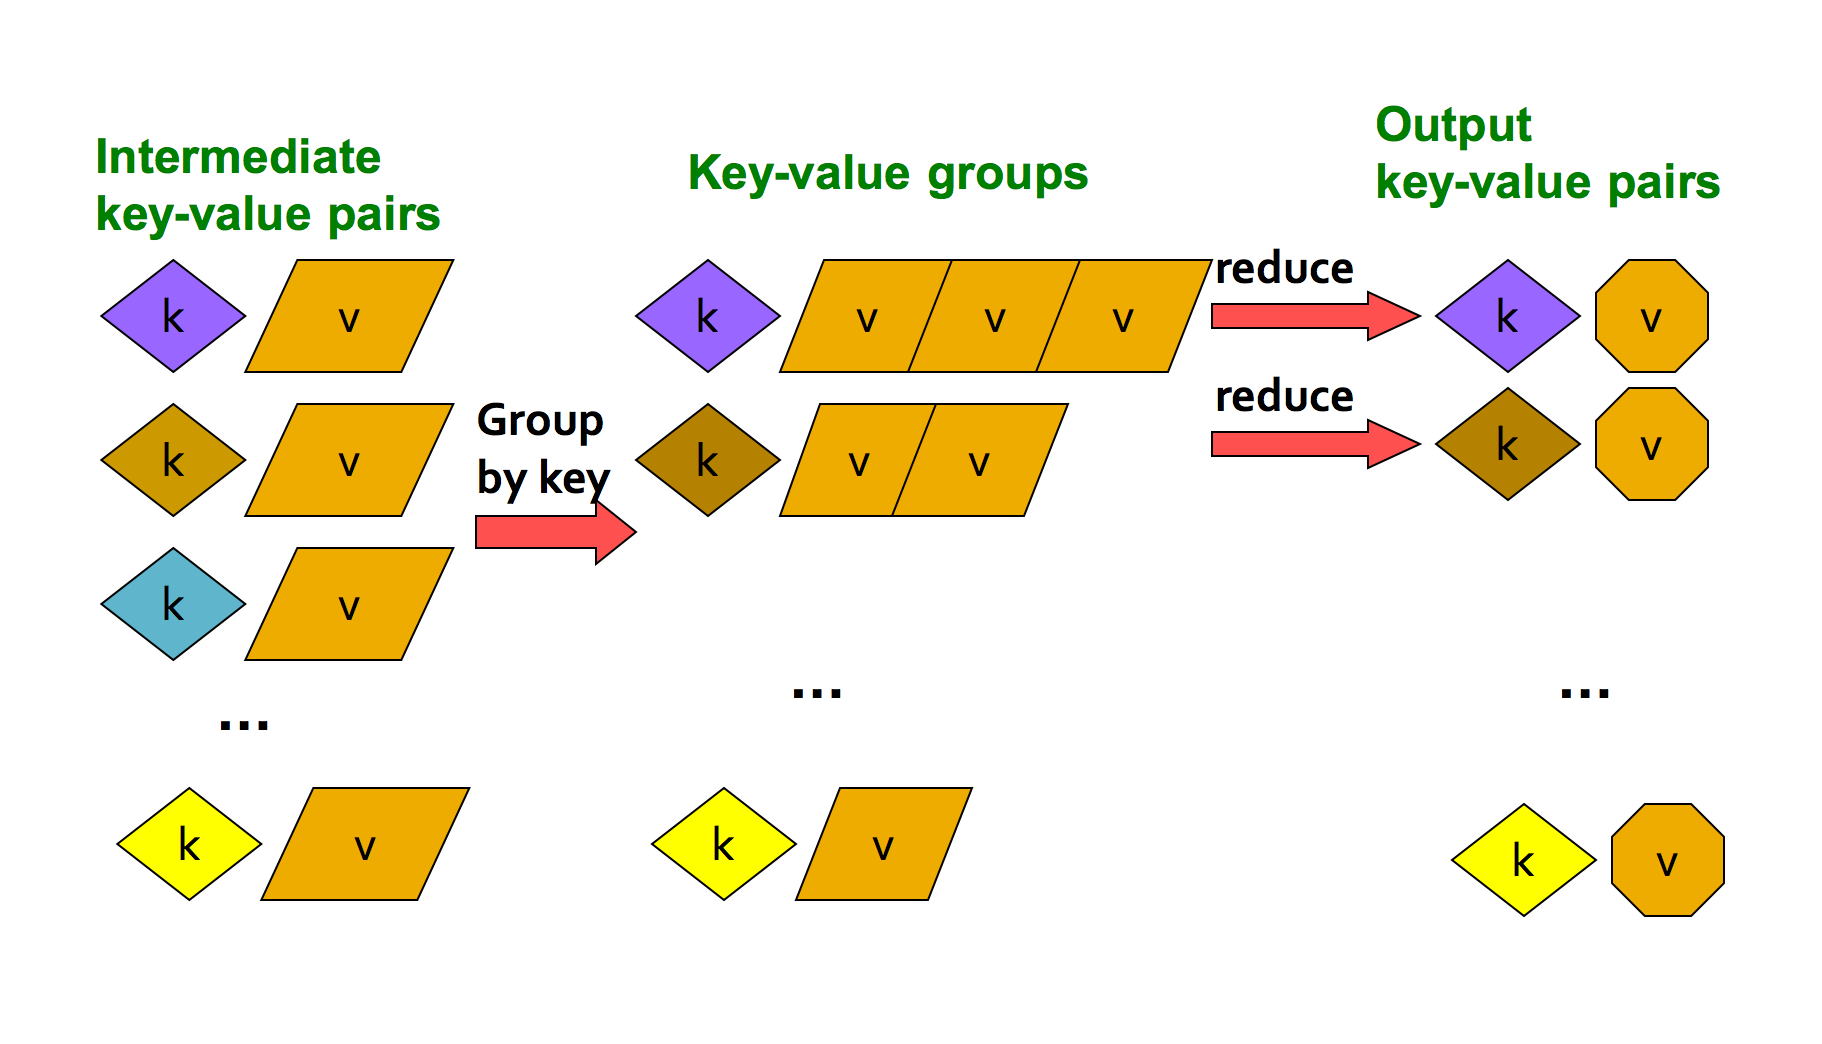
\includegraphics[width=.95\textwidth]{img/mapreduce.png}
% \end{figure}
% shamelessly stolen from CS246
% \end{frame}

% \begin{frame}
% \frametitle{Classic example: Word Count}
% Take a large file and output the counts of each word in that file.

% \vfill\pause

% We'll input each line of the file into our mappers as values, ignoring the key.
% From each mapper we'll emit pairs consisting of (word, 1).

% \vfill\pause

% The reducer will take keys and get a list of 1's as values which we will
% sum to get each word count.
% \end{frame}

% \begin{frame}
% \frametitle{Classic example: Word Count}
% \begin{figure}[h]
% \centering
% 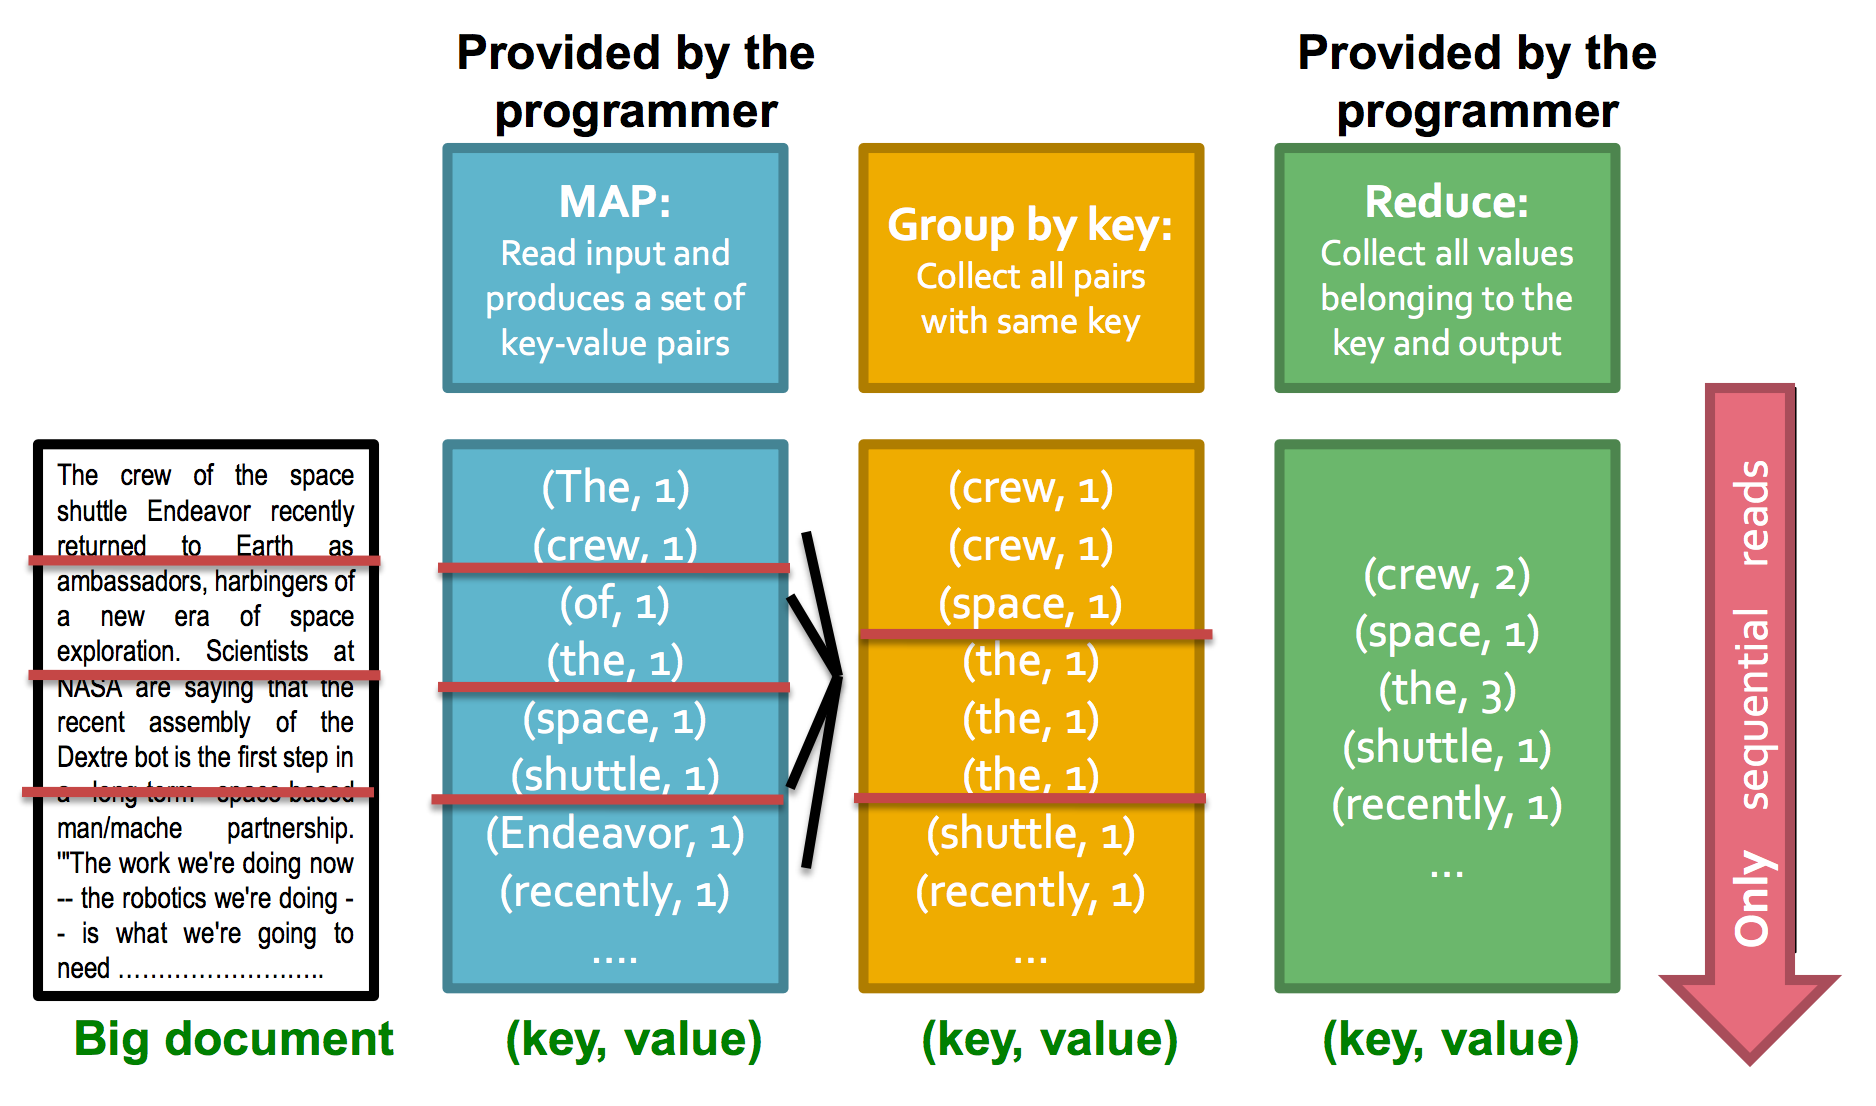
\includegraphics[width=.95\textwidth]{img/wordcount.png}
% \end{figure}
% shamelessly stolen from CS246
% \end{frame}

% \begin{frame}
% \frametitle{Mapper for WordCount}
% Take in one \texttt{(\_, line\_of\_text)} pair and output \text{(word, 1)} pairs
% \codeblock{code/mr_mapper.py}
% \end{frame}

% \begin{frame}
% \frametitle{Reducer for WordCount}
% Take in one \texttt{(word, list\_of\_ones)} pair and output  \text{(word, sum)} pair
% \codeblock{code/mr_reducer.py}
% \end{frame}


%     \begin{frame}\frametitle{Dumbo}
%         \framesubtitle{\url{https://github.com/klbostee/dumbo/wiki}}

%         The above was an abstract overview of the Map Reduce paradigm.

%         \vfill

%         Mostly written using Java. However, possible to write in Python, for
%         example using \emph{Dumbo} (or \emph{Streaming}).

%         \vfill

%         Dumbo is a very convenient Python API to write Map Reduce programs

%     \end{frame}

%     \begin{frame}\frametitle{Spark}
%         \framesubtitle{\url{http://spark.apache.org/}}

%         `New generation of MapReduce implementation'

%         \vfill

%         Keeps data in memory, therefore much faster.

%         \vfill

%         Mostly in Scala, but can also be used with Python.

%         \vfill

%         Libraries: Shark (SQL), Streaming, GraphX, MLLib

%     \end{frame}


% % section more_modules (end)
